\documentclass{beamer}
\graphicspath{{./figures/}} 
\mode<presentation>
{
  \usetheme{default} 
  \usecolortheme{default}
  \usefonttheme{default}
  \setbeamertemplate{navigation symbols}{}
  \setbeamertemplate{caption}[numbered]
} 

\usepackage[portuguese]{babel}
\usepackage[utf8]{inputenc}
\usepackage{graphicx}

\title[]{Pesquisa de Algoritmo Estocástico para o Problema U-Curve}
\author{Gustavo Estrela}
\institute{Universidade de São Paulo e Texas A\&M University}
\date{\today}

\begin{document}

\begin{frame}
  \titlepage
\end{frame}

\section{Objetivo}
\begin{frame}{Objetivo}
\begin{itemize}
  \item Estudo do algoritmo IUBB.
      \vskip 5em
  \item Implementação de uma variante estocástica do IUBB.
\end{itemize}
\end{frame}

\section{O Algoritmo IUBB}
\begin{frame}{O Algoritmo IUBB}
    \begin{itemize}
        \item{Baseado no UBB.}
        \vskip 5em
        \item{Duas ideias principais:}
        \begin{itemize}
            \vskip 1em
            \item{Atualização iterativa de cadeias ótimas.}
            \vskip 1em
            \item{Uso da bisecção na procura do mínimo de uma cadeia.}
        \end{itemize}
    \end{itemize}
\end{frame}

\section{Introdução do erro}
\begin{frame}{Introdução do erro}
    \begin{itemize}
        \item{Assumimos erro com distribuição normal com média zero e
            variância $\sigma^2$.}
        \item{Efeitos do erro no algoritmo IUBB.}
        \begin{figure}[h]
            \includegraphics[page=15, clip, trim=12cm 10.7cm 3cm 12cm,
                scale=.8]{IUBB_submit}
            \caption{Efeito de um erro senoidal nos algoritmos UBB e 
                IUBB \cite{iubb}}
        \end{figure}
    \end{itemize}
\end{frame}

\section{Algoritmo Tradicional de Bisecção}
\begin{frame}
    \begin{itemize}
    \end{itemize}
\end{frame}

\section{Algoritmo de Bisecção Mid-neighbour}
\begin{frame}{Algoritmo de Bisecção Mid-neighbour}
    \begin{itemize}
        \item{Não usa informação sobre o erro.}
        \item{Conceito de confiança sobre a diferença observada entre
            vizinhos.}
    \end{itemize}
\end{frame}

\section{Referências}
\begin{frame}{Referências}
\begin{thebibliography}{9} \label{sec:referencias}
\addcontentsline{toc}{section}{Referências}
\bibitem{msreis thesis}
Reis, Marcelo S. ``Minimization of decomposable in U-shaped curves 
functions defined on poset chains–algorithms and applications." PhD
thesis, Institute of Mathematics and Statistics, University of São 
Paulo, Brazil, (2012).
\bibitem{ucs paper}
Reis, Marcelo S., Carlos E. Ferreira, and Junior Barrera. ``The U-curve
optimization problem: improvements on the original algorithm and time
complexity analysis." arXiv preprint arXiv:1407.6067, (2014). 
\bibitem{iubb}
Atashpaz-Gargari, Esmaeil, Ulisses M. Braga-Neto, and Edward R.
Dougherty. ``Improved branch-and-bound algorithm for U-curve 
optimization." 2013 IEEE International Workshop on Genomic Signal
Processing and Statistics (GENSIPS), (2013).
\end{thebibliography}
\end{frame}

\end{document}

